\subsection{\label{source}{\color{OliveGreen}PASS}:
Flow created by a cilindrical volume source
}
\cutname{source.html}
\begin{description}
\item[Author]Daniel Fuster
\item[Command]{\tt sh source.sh source.gfs}
\item[Version]1.3.2
\item[Required files] source.gfs \htmladdnormallinkfoot{(view)}{source/source.gfs.html} \htmladdnormallinkfoot{(download)}{source/source.gfs}\\ \htmladdnormallinkfoot{source.sh}{source/source.sh} \htmladdnormallinkfoot{source.gfv}{source/source.gfv} \htmladdnormallinkfoot{error.gfv}{source/error.gfv}
\item[Running time] 27 seconds
\end{description}

The flow created by a cilindrical volume source is compared
against the analitical solution.

u_r = { s r \over 2 } \; \; if \; \; r \le R_c
u_r = { s R_c^2 \over 2 r} \; \; if \; \; r > R_c

\begin{figure}[htbp]
\caption{\label{Velocity Norm} Velocity field.}
\begin{center}
\includegraphics[width=\hsize]{source/velfield.eps}
\end{center}
\end{figure}

\begin{figure}[htbp]
\caption{\label{Error Norms} Error Norms.}
\begin{center}
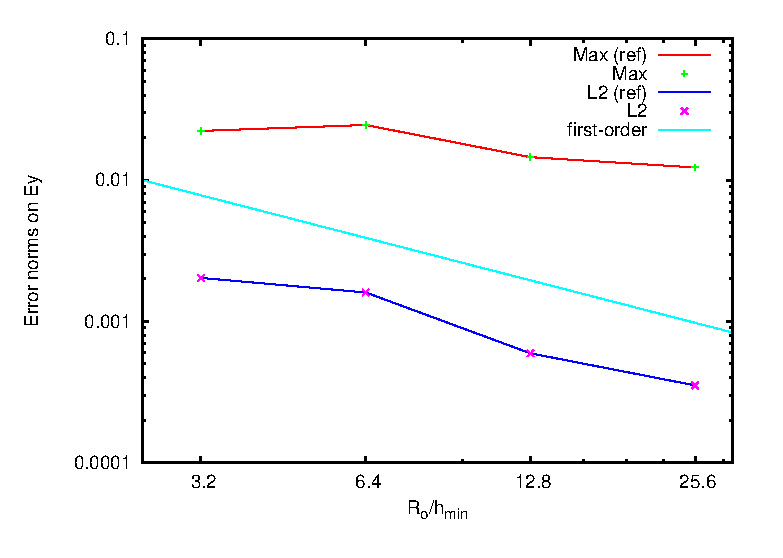
\includegraphics[width=\hsize]{source/error.eps}
\end{center}
\end{figure}

\begin{figure}[htbp]
\caption{\label{Relative Local Error} Local error at level 13. Color scale [-5e-4:5e-4].}
\begin{center}
\includegraphics[width=\hsize]{source/localerror.eps}
\end{center}
\end{figure}
